
\documentclass{TDP005mall}
\usepackage{pdfpages}
\usepackage{graphicx}

\newcommand{\version}{Version 1.2}
\author{Josefin Bodin\\
  Alicia Bergman \\
Ahmed Sikh}
\title{Kravspecifikation}
\date{\today}
\rhead{Josefin Bodin\\
  Alicia Bergman\\
Ahmed Sikh}



\begin{document}
\projectpage
\section{Revisionshistorik}
\begin{table}[!h]
\begin{tabularx}{\linewidth}{|l|X|l|}
\hline
Ver. & Revisionsbeskrivning & Datum \\\hline
1.3 & Kompletterat utifrån handledarens feedback & 201129 \\\hline
1.2 & Visualisering tillagd & 201120 \\\hline
1.1 & Kompletterat utifrån feedback & 201118 \\\hline
1.0 & Första utkast & 201117 \\\hline
\end{tabularx}
\end{table}

\label{prereq}
\section{Spelide}
ME WANT COOKIE!!\\
Detta labyrintspel går ut på att leta sig igenom labyrinten för att nå mitten av
spelplanen. Spelaren gestaltas av ett kakmonster och på vägen in mot mitten kan man
samla poäng genom att äta de kakor man stöter på. Men se upp för de brända då de
slukar poäng samtidigt som du slukar dem. Du måste även akta dig för de onda
grönsakerna som rör sig runt spelplanen och bara väntar på att ta ett av
spelarens liv. Fienderna rör sig i ett bestämt mönster så ibland kan lite
tålamod hjälpa spelaren. Vid eventuell kollision med en fiende förlorar spelaren
ett liv och fienden försvinner från spelplanen. Man har totalt tre liv och
förlorar man dem alla så tar spelet slut utan att man får ta hem någon
vinst. Detta är ett high score spel och varje kvarvarande liv ger 10 poäng när
spelaren når mitten, så varje hjärta gäller.


\section{Målgrupp}
Spelet är menat för alla som vill ha en inte allt för avancerad tidsfördriv. 

\section{Spelupplevelse}
Detta är ett enkelt spel där tålamod triumferar över stress och man kan själv
välja om målet är att samla så många poäng som möjligt eller bara leta sig in
till mitten.

\section{Spelmekanik}
Spelaren rör sig genom labyrinten med hjälp av piltangenterna och man kommer
endast kunna röra sig i riktningarna upp, ned, höger och vänster. 

\newpage

\section{Regler}
\subsection{Spelplan}
Spelplanen kommer vara en labyrint sedd ovanifrån och storleken
kommer vara densamma som skärmen. Utrymmet mellan väggarna där spelaren kommer
röra sig kommer inte vara mycket större än spelaren och det går självklart inte
att röra sig genom väggarna.

\subsection{Spelare}
Spelaren kommer gestaltas av ett kakmonster och börjar med 3 liv. Spelaren
förlorar ett liv vid kollision med en fiende och när alla liv gått förlorade är
spelet slut och man har förlorat. Spelaren ska röra sig från utsidan av
labyrinten in till mitten och kan röra sig i riktningarna upp, ned, höger och
vänster.

\subsection{Poäng/liv}
Spelaren kan under spelets gång samla poäng genom att äta kakor som ligger
utplacerade på olika plateser i labyrinten. En kaka ger 5 poäng. Råkar man
dock äta en bränd kaka förlorar man 3 poäng. Poängen kommer synas uppe i
höger hörn och liven i form av hjärtan i vänster hörn.


\subsection{Fiender}
I detta spel är grönsakerna dina fiender. De rör på sig utmed en bestämd rutt
och om spelaren stöter på dem förlorar hen ett liv och fienden
försvinner. Det kommer finnas minst två fiender med lite andra egenskaper. Det
ena kommer att explodera och tilldelar mer i skada och spelaren förlorar 2 liv
istället för ett. Den andra kommer att skjuta objekt på spelaren och den tredje
kommer endast vandra sin förutbestämda rutt.



\section{Visualisering}

\begin{figure}
  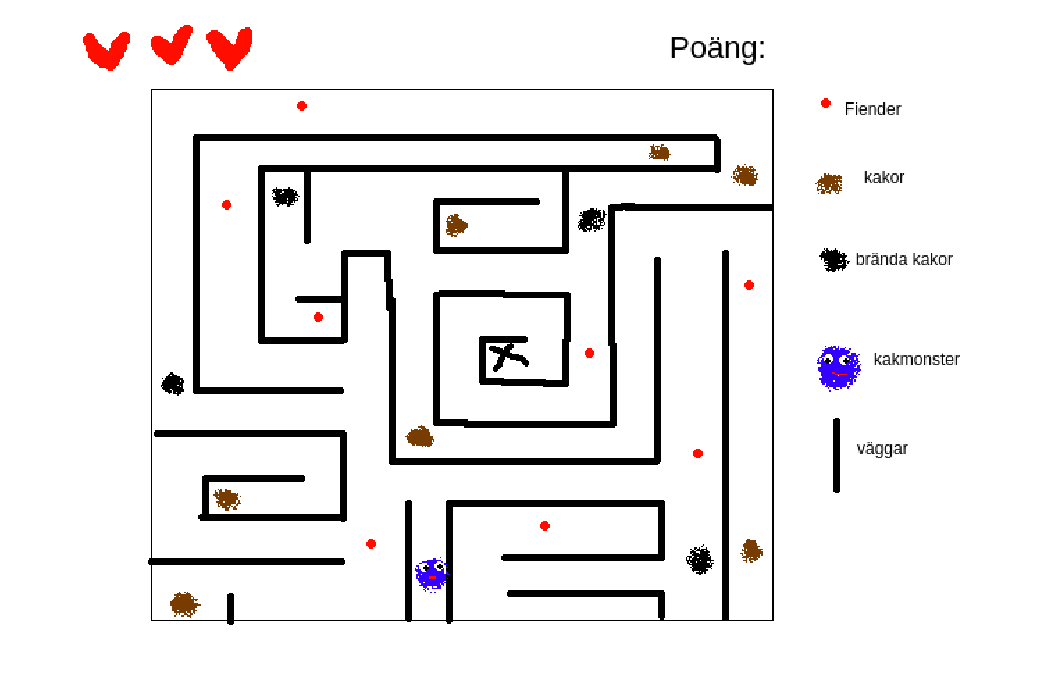
\includegraphics[scale=0.5]{Banavis.png}
  \caption{Spelplan}
  \label{fig:game}
\end{figure}

Figur \ref{fig:game} visar en lofi-prototyp för hur banan kan komma att vara utformad. Kakor och
brända kakor kommer vara utplacerade på banan och fiender kommer vandra i ett
bestämt mönster. Spelarens uppgift är att ta sig till mitten med så många poäng
som möjligt och livet i behåll.

\newpage

\section{Kravformulering}
\subsection{ska-krav}
\begin{enumerate}
\item 2D spelplan, Användaren ska se en labyrint i fågelvy.
\item Användare styr en spelare i form av ett kakmonster.
\item Spelaren ska undvika fiender som ska ha en design av grönsaker. Exempel på fiender är en formad som en morot och en chili.
\item Kakor utplacerade på spelplanen ger 5 poäng vid kollision.
  \item Kakorna skall vara strategiskt utplacerade på spelplanen.
\item Brända kakor utplacerade på spelplanen ger -3 poäng vid kollision.
\item Det ska finnas minst en fiende som rör sig i bestämt mönster. Den har en rutt som den följer.
\item Morötterna rör sig i ett bestämt mönster och ger -1 liv vid kollision.
  \item Chilin rör sig i bestämt mönster och exploderar när spelaren är inom en specifik räckvidd och ger -2 liv. 
\item Användaren styr spelaren med tangenterna a, w, s och d i riktningarna w = upp, s = ned, d = höger och a = vänster.
\item Kakor och fiender försvinner vid kollision med spelaren. Fienderna ger då även skada och kakorna ger eller tar poäng.
\item Det ska finnas en startmeny där det ska finnas möjlighet att starta och stänga spelet.
\item Banan ska vara lika stor som fönstret.
  \item Spelaren ska inte kunna gå genom väggar. Vid kollision kommer inte spelaren kunna röra sig i den riktningen.

\subsection{bör-krav}
  \item Ett minst antal fiender på spelplanen(en fiende försvinner, en annan
    tillkommer).
  \item Det finns olika typer av kakor som ger olika mycket med poäng och kakor som har egenskaper som låter spelaren passera genom fiender utan att förlora liv.
  \item Potions finns på spelplanen som ger ett liv till spelaren om den har förlorat något liv tidigare i spelet.
  \item En fiende i form av en ärtskida som skjuter ärtor på spelaren.
    \item Det finns en sida där användaren kan se poängställningen och den kan öppnas via startmenyn.
  \end{enumerate}


\section{Kravuppfyllelse}

    \textbf{Spelet ska simulera en värld som innehåller olika typer av objekt. Objekten
    ska ha olika beteenden och röra sig i världen och agera på olika sätt när de
    mäter andra objekt.}\\
    \emph{Uppfylls av krav: 1,4,6,8,9}
    
    \textbf{ Det måste finnas minst tre olika typer av objekt och det ska finnas flera
    instanser av minst två av dessa. T.ex ett spelarobjekt och många instanser
    av två olika slags fiendeobjekt.}\\
    \emph{Uppfylls av krav: 2,3,4,6,8,9}
    
    \textbf{Ett beteende som måste finnas med är att figurerna ska röra sig över
    skärmen. Rörelsen kan följa ett mönster och/eller vara slumpmässig. Minst
    ett objekt, utöver spelaren ska ha någon typ av rörelse.}\\
    \emph{Uppfylls av krav: 3,8,9}
    
    \textbf{En figur ska styras av spelaren, antingen med tangentbordet eller med
    musen.}\\
    \emph{Uppfylls av krav: 2,10}
    
    \textbf{Grafiken ska vara tvådimensionell.}\\
    \emph{Uppfylls av krav: 1}
    
    \textbf{Världen (spelplanen) kan antas vara lika stor som fönstret.}\\
    \emph{Uppfylls av krav: 13}
    
    \textbf{Det ska finnas kollisionshantering, det vill säga, det ska hända olika saker
    när objekten möter varandra, de ska påverka varandra på något sätt. T.ex kan
    ett av objekten tas bort, eller så kan objekten förvandlas på något sätt,
    eller så kan ett nytt objekt skapas.}\\
    \emph{Uppfylls av krav: 4,6,8,11,14}
    
    \textbf{Det ska vara enkelt att lägga till eller ändra banor i spelet. Detta kan
      exempelvis lösas genom att läsa in banor från en fil}\\
    \emph{Uppfylls av krav: 12}
    
    
    \textbf{spelet måste upplevas som ett sammanhängande spel som går att
      spela!}\\
    \emph{Uppfylls av alla krav}
    

\end{document}
